% Eights pages allowed total
\documentclass[sigconf, nonacm]{acmart}

\usepackage{booktabs} 
\usepackage{amsmath}
\usepackage{subfigure}
\usepackage{multirow}
\usepackage{xcolor}
\usepackage{hyperref}

\begin{document}
\title{Mitigating Batch Effects and Enhancing Cooperativeness Classification in Human Survey Data}

\author{Konghao Zhao}
\authornote{Both authors contributed equally to this research.}
\affiliation{%
   \institution{Wake Forest University}
   \streetaddress{1834 Wake Forest Road}
   \city{Winston Salem}
   \state{North Carolina}
   \country{USA}
 }
 \email{zhaok220@wfu.edu}
 
 \author{Cade Wiley}
 \authornotemark[1]
\affiliation{%
   \institution{Wake Forest University}
   \streetaddress{1834 Wake Forest Road}
   \city{Winston Salem}
   \state{North Carolina}
   \country{USA}
 }
 \email{wilecr18@wfu.edu}

 \author{Natalia Khuri}
\affiliation{%
   \institution{Wake Forest University}
   \streetaddress{1834 Wake Forest Road}
   \city{Winston Salem}
   \state{North Carolina}
   \country{USA}
 }
 \email{khurin@wfu.edu}

\begin{abstract}
% The title of the study is “Mitigating Batch Effects and Enhancing Cooperativeness Classification in Human Survey Data” and it is authored by Konghao Zhao and Cade Wiley from Wake Forest University. This study explores how to eliminate batch effects in a dataset and how to use data augmentation to improve the performance of classifiers, specifically to identify high fidelity data. The dataset used in this study is “The Attack on America and Civil Liberties Trade-Offs: A Three-Wave National Panel Survey, 2001-2004” produced by Darren Davis and Brain Silver. Ultimately we conclude that data augmentation is productive for improving the performance of classifiers to identify high fidelity data. The main contributions of this study are an automated framework for benchmarking data augmentation techniques, a framework using data augmentation techniques to generate high fidelity training data, and a classifier for predicting the cooperativeness of survey respondents.
The quality of a survey largely depends on how respondents respond to the question, and an inferior response generated by a lack of cooperation might severely deteriorates the quality of the survey. However, identifying subjectively whether a respondent is cooperative or not is a challenging problem. This study focuses on enhancing the classification of respondent cooperativeness in a survey data. To identify high fidelity data and improve the performance of classifiers, the study addresses the challenges of noisy, imbalanced, and biased data through well-structured data processing pipelines, augmentation methods, and a data transformation method. We conclude that data augmentation is productive for improving the performance of classifiers and our proposed data transformation could mitigate the batch effects. The contributions of this study are an automated framework for benchmarking data augmentation techniques and generating high fidelity training data, a good performing classifier for predicting the cooperativeness of survey respondents, and a data transformation method to mitigate the batch effect.
\end{abstract}

\maketitle
\section{Introduction}\label{sec:introduction}
\begin{figure*}[t!]
    \centering
    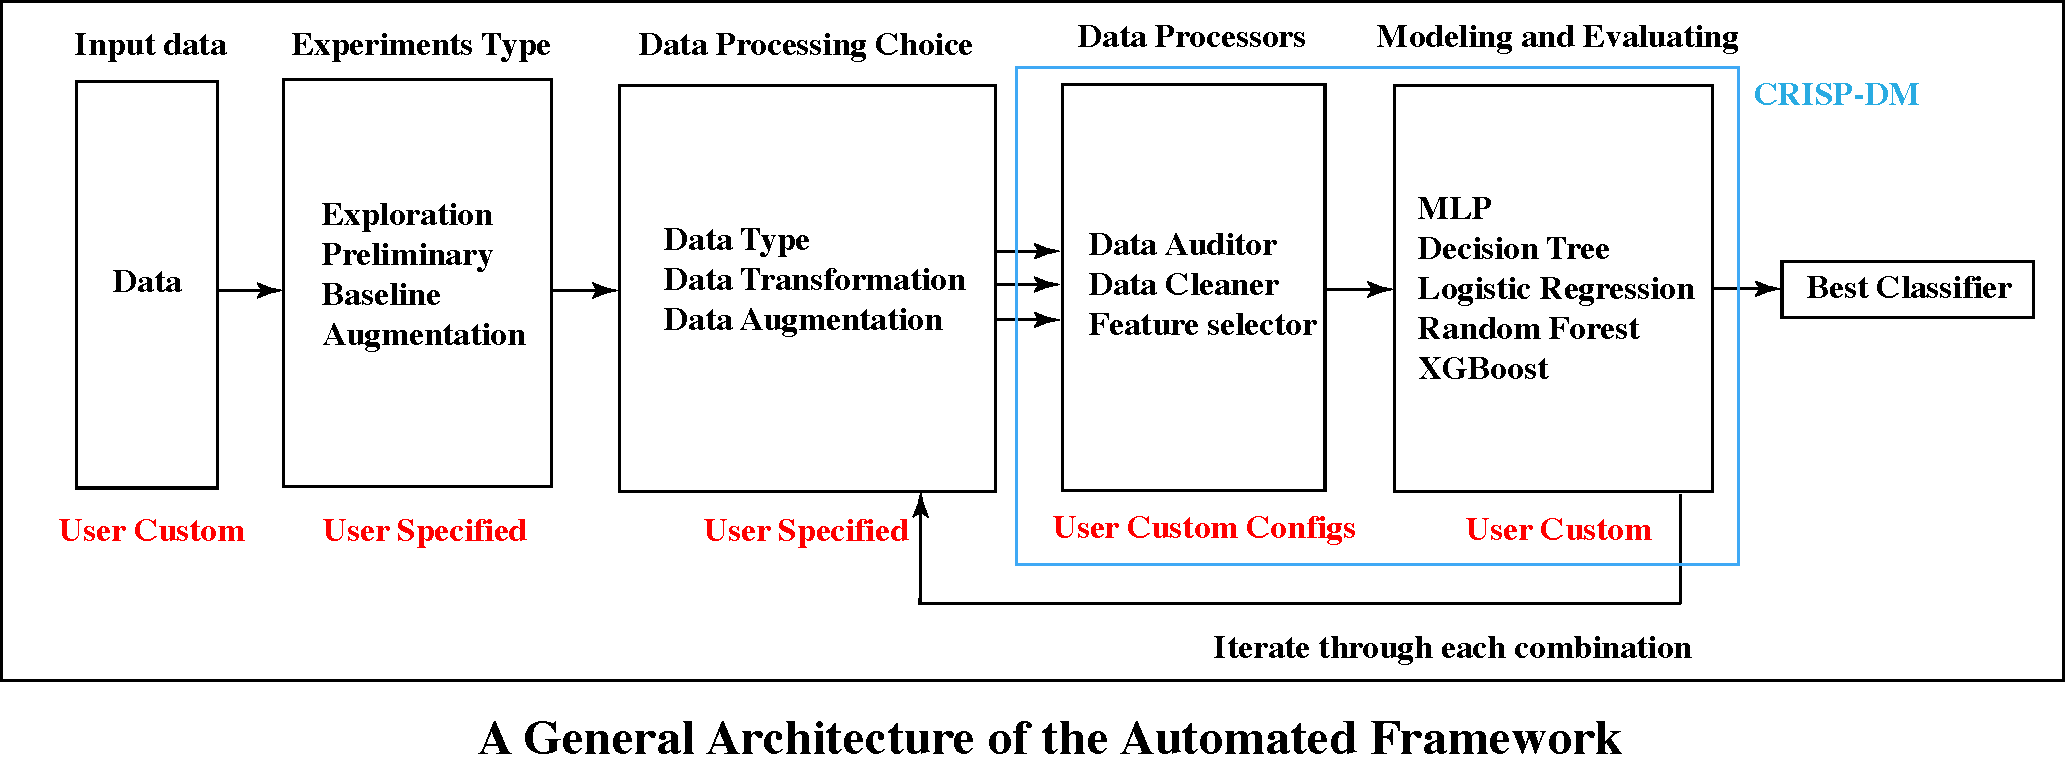
\includegraphics[width=\linewidth]{Figures/Figure1.pdf}
    \caption{A general architecture of the automated framework. The main steps for using this framework contain the following steps: 1. choose the dataset to use, 2. choose the type of benchmarking experiments to run, 3. specify which combination of data processing choice to use, 4. iterate through CRISP-DM process for each combination of data processing choice to explore the best classifier.}
    \label{fig:figure1}
\end{figure*} 

Identifying cooperative survey respondents is an important task since many surveys risk processing falsified data by taking untruthful responses seriously. This is particularly true for interviews taking place over technology where respondents may not feel as accountable for their responses. In our study we explored how to build a good performing classifier to classify the cooperativeness of the respondents, where its performance is aimed to be improved by data augmentation and transformation methods. To classify the cooperativeness, specific to our dataset ``The Attack on America and Civil Liberties Trade-Offs: A Three-Wave National Panel Survey, 2001-2004'' ~\cite{data}, we used a feature that tracks cooperativeness to be an indicator of the quality of the responses. When a respondent has a high cooperation level, we assume that data is of high quality and should be processed. 

Throughout our experiments, we faced three major challenges. Our dataset contained noisy, imbalanced, and biased data. To address the noisiness of our dataset we developed a series of data processing pipelines to reduce noise which we describe in Data Processing section of Data and Methods. To address the class imbalances, we employed a variety of data augmentation methods which we have compared the effectiveness of in our results section. To reduce the batch effects also referred to as data bias, we removed the variables causing the batch effect and proposed a data transformation method to reformat the dataset in a denser representation better fit for machine learning classifiers. 

Our study makes contributions to benchmarking data augmentation methods, generating high fidelity data, and mitigating batch effects of the data. We designed and implemented a user-friendly and automatic framework to benchmark data augmentation methods, with a reproducible data processing pipeline to create data. Using data augmentation methods to generate high fidelity training data, we created a classifier that predicts respondents’ cooperativeness during the interview with high performance. We also proposed a data transformation method to mitigate the batch effect, or form of data bias, found in our dataset. 
\begin{table}[!t]
\caption{Table of size of training data with and without data augmentation methods. The size of testing data (684, 226) is the same regardless of the methods. The size is doubled when the sample-based methods are augmented with GAN.}
\label{tab:table1}
\scalebox{0.68}{
\begin{tabular}{lcccccc}
\toprule
              & Baseline & SMOTE & editENN  & TomekLinks & SMOTEENN & SMOTETomek \\ \hline
Untransformed & 1044(684)       & 2184  & 1044 & 1044       & 1058     & 2082       \\
Transformed   & 360(226)        & 638   & 192  & 360        & 166      & 552        \\ \bottomrule
\end{tabular}
}
\end{table}
\section{Related Works}
\subsection{The Attack on America and Civil Liberties Trade-Offs}
Since the formation of our dataset “The Attack on America and Civil Liberties Trade-Offs: A Three-Wave National Panel Survey, 2001-2004” has been collected ~\cite{data}, there have been over ten publications based on the data. Most publications are descriptive, where researchers are looking to explain patterns in the data, while few are methodological, where researchers are explaining steps taken during data collection. 

The most notable publications come directly from the original authors Davis and Silver. Davis and Silver study the willingness of individuals to give up civil liberties or security based on their ethnicity, political affiliation, trust in government, and sense of fear ~\cite{Davis_Silver_2004_1}. While they found many detailed relationships in the data, overall they discovered that Americans’ commitment to democratic values is highly contingent on a range of factors and that large-scale threats significantly impact an individual’s willingness to give up their rights. In a similar study ~\cite{Davis_2004_2}, Davis and Silver look specifically at the relationship between ethnicity and individuals’ responses to the 2001 September 11 attacks. Davis and Silver found that Latinos, Whites and African Americans all rallied around political leaders and the United States; however, each ethnicity had varying rates of supporting democratic values and evaluating the United States as partially responsible for the 2001 September 11 attacks. 

In addition, Davis and Silver analyze the dataset for political trends. They study what Americans perceived was the cause of the 2001 September attacks, where they found that 53 percent of Americans saw the United States as somewhat responsible~\cite{Davis_Silver_2004_3}. In ~\cite{Davis_Silver_2004_4}, Davis and Silver analyze whether the perceived threat surrounding terrorism from 2001 to 2004, influenced Americans' support of President George Bush. Ultimately, they conclude that the more individuals feared terrorism, the less likely they were to support Bush’s presidency.

While all these studies yield meaningful results about the data, there are no publications focused on using this dataset to identify untrustworthy survey responses. In our study, we focus on developing a classifier to identify untrustworthy survey responses to better provide higher fidelity data.

\subsection{Data Augmentation Methods}
Data augmentation refers to the techniques used to artificially increase the size of a dataset via a set of transformations applied to the original dataset. Data augmentation methods have recently been most popular within image and text data; however, they have been applied to a wide range of data types including tabular data. For image data, geometric, color and spatial transformation are often popular as it allows for one image to generate many samples ~\cite{Khoshgoftaar_2019}. 

Sampling techniques, generative models, and noise injection are popular for tabular data. Sampling techniques, such as SMOTE, aim to diversify the data by maintaining a balanced representation of the different classes ~\cite{SMOTE_Kegelmeyer_2002}. Generative models, such as Generative Adversarial Networks (GANs) or Variational Autoencoder (VAE), use neural networks to generate realistic artificial samples ~\cite{Meor_Yahaya_Teo_2023, Sandfort_Yan_2019}. In addition to generative modeling data augmentation, recently contrastive learning based and masked modeling based data augmentation methods have become popular for tabular data. VIME ~\cite{Yoon_2020} and SCRAF ~\cite{Bahri_2021} are examples of masked modeling based data augmentation methods and SubTab ~\cite{Ucar_2021} and Transtab ~\cite{Wang_Sun_2022} are contrastive learning based data augmentation methods. Some studies have started to use transformers for data augmentation such as FeatMix ~\cite{Chen_Yan_Chen_Wu_2023} and HiddenMix ~\cite{Chen_Yan_Chen_Wu_2023}. While these are the most relevant data augmentation techniques for our study, the field of data augmentation has a wide range of rapidly developing approaches. 
\section{Data and Methods}\label{sec:data\_and\_methods}

\subsection{General Architecture of the Framework}
Figure 1 demonstrates the implementation of our workflow. The first step of our workflow, input data, asks the user to input their data. While our workflow was developed specifically in reference to “The Attack on America and Civil Liberties Trade-Offs: A Three-Wave National Panel Survey, 2001-2004”, many aspects of the workflow are fully reusable for other datasets. 

In the second stage, the user sets their specifications that corresponds to the type of experiment they would like to run choosing from one of the following options: exploration, preliminary, baseline, or augmentation. For each of the experiment choice, a result file will be output in this own directory in the output directory for examination. 

In the following workflow step, data processing choice, the user specifies what data type they would like to store their data in if they want their data transformed, and if or how they want their data to be augmented. If the experiment type is exploration, user can choose whatever combination to explore. If the choice is preliminary, the workflow will automatically executes experiments for discovery of batch effects. Baseline and augmentation choice will enable the workflow to automatically combine all data processing choice and perform benchmarking studies. 

In data processors, the data moves through the data auditing pipeline, the data cleaning pipeline, and the feature selection pipeline. Next is the modeling stage, where all of the classifiers are trained with the data input from the data processor stage. During these two stages, users can also set their preferred data processing threshold and hyperparameter tuning values in the configuration file. 

After the classifiers have been trained the best classifier can be selected from the results. A cycle in the workflow was drawn to show that the workflow was developed so that users could iteratively develop classifiers with different inputs and specifications to yield a high performance model with high fidelity data. 

\subsection{Data Description}
The original shape of our dataset is 3361 by 787 where there are 3361 samples and 787 features. After processing our data and preparing it for our classifiers, the size of our dataset decreases significantly. In Table 1, we compare the size of our training dataset across data augmentation methods with and without our proposed data transformation specific to the dataset. Without the transformation, the dataset contains many more samples. At the baseline comparison, the untransformed dataset has near three times the samples as the transformed dataset. While the ratio between the number of untransformed training dataset size and transformed training dataset size varies, the untransformed dataset contains significantly more samples across all data augmentation methods. Interestingly, since we employed a variation of data augmentation methods, including undersampling, not all data augmentation methods resulted in a training dataset larger than the baseline. In editENN and SMOTEEEN, the size of the training dataset decreased for the transformed iteration. We also found a existence of batch effect in our dataset. Batch effect occurs when variations in data that are not related to their actual labels but a dominant feature, underlying structure make it difficult to analyze the data of interest. 

\subsection{Data Transformation}
To transform the original data format into a format well suited for classifiers and remove batch effects, we decreased the number of attributes associated with each respondent. In its original form, each sample is associated with 787 attributes. However, 91 wave dependent variables record the same data for different waves of the survey. To reduce the number of attributes we condensed these three sets of wave dependent attributes into one set of wave dependent variables. This left us with 515 attributes per column. With 515 attributes we are able to represent a respondent and one of the respondents responses in a survey wave. Rather than keep all of the survey waves for each respondent, we only kept the wave in which the respondent participated. This left us with a much denser dataset. Rather than having 91 to 192 attributes filled with null values for each respondent, we instead have 515 attributes with few null values. After the data transformation, the shape of our transformed dataset is 3661 by 515.

\subsection{Data Processing}
During data processing, the data moves through three pipelines ultimately yielding the processed data in four formats for the user to choose from, Raw data, PCA components, UMAP components, UMAP\_PCA components. Our pipelines are designed to serve a specific function, where the first pipeline is for auditing the data, the second pipeline for cleaning the data, and the last pipeline for feature selection. Our data audit pipeline is designed to produce a report to the user with useful information about the data. The pipeline contains the following five steps: note duplicate rows, note duplicate columns, note columns with a null percentage above a user defined threshold, and note rows with a null percentage above a user defined threshold. All the irregular indices of rows and columns are stored in a dictionary that could be later accessed by the data cleaning pipeline. Although our data audit pipeline makes note of useful information for the user it does not make any changes to the data.

In our data cleaning pipeline, we make changes to the data that were identified in our data audit pipeline. The data cleaning pipeline is made up of four steps as follows: delete columns with a null percentage above a user defined threshold, delete duplicate columns and rows, and delete outlier rows with a user defined standard deviation threshold. After our data has been cleaned, we send our data to our final pipeline, the feature selection pipeline. We defined the standard deviation threshold at 3 standard deviations and the maximum null percentage at 0.4 for all the experiments.

The feature selection pipeline takes input from data cleaning pipeline and is made up of the following steps: stratify balance data upon a user defined label column, remove correlated features above a user defined threshold by computing the correlation matrix, exclude the one feature from the correlating pair, normalize the columns using Min-Max scaling, and perform variable feature selection obtaining the top standard deviation of 100 features. If the size of the features is smaller than 100, the original features are obtained. After the data has passed through the feature selection pipeline, it will be ready to be processed as Raw data, or be converted to either PCA or UMAP components. In our implementation we balance the data upon W3IWER4\_A which is the target variable. We set the feature correlation upper bound at 0.98 and set the number of variable features to select to 100.

Ultimately, the user has four choices on the format of the data which they would like to process. As mentioned previously the four formats are Raw, PCA components, UMAP components, UMAP\_PCA components. We included PCA components to allow users to try to find linear patterns in their data. Additionally, we included UMAP components to allow users to find non-linear patterns in their data. We also included UMAP\_PCA components since this is often a technique in exploratory data analysis. Lastly, we included Raw data for datasets like ours that were small enough to be processed without dimensionality reduction. We provide different means to provide user a better flexibility to explore the relationship within the dataset and to improve the visualizations. 

\subsection{Data Augmentation Methods}
In our study, we explore various data augmentation methods to address the issue of class imbalance in our training dataset. Five primary sampling-based techniques are employed, including over-sampling, under-sampling, and hybrid-sampling methods. Additionally, we integrate a Generative Adversarial Network (GAN) with each method, effectively doubling the size of the training dataset. Therefore, in total, we tested 10 data augmentation methods on our dataset.

\subsubsection{Synthetic Minority Over-sampling Technique (SMOTE)}
SMOTE is a widely-used benchmarking approach for upsampling imbalanced datasets ~\cite{SMOTE_Kegelmeyer_2002}. It works by creating synthetic samples for the minority class, thus balancing the distribution of classes. It is an iterative method that first selects a minority class, identifies the k-nearest neighbors, and at last, generates synthetic instances within the same neighborhood.

\subsubsection{Edited Nearest Neighbour (editENN)}
EditENN focuses on improving the quality of the training set by removing instances that may be noise or are likely misclassified ~\cite{Wilson_1972}. It does this by considering the nearest neighbors of each instance. That is, if an instance's class label differs from the majority of its neighbors, it is removed. This method helps in cleaning the data and can lead to a more balanced class distribution. Although editENN modifies the majority class, it preserves the samples in the minority class to maintain its integrity.

\subsubsection{Tomek’s links (TomekLinks)}
Like editENN, Tomek-Links also modify the majority class to improve model generalization ~\cite{Elhassan_M_2016}. Tomek-Links are pairs of samples, one from the majority class and one from the minority class, that are nearest neighbors. After the Tomek-Links have been identified, the Tomek-Links samples in the majority class are removed. The motivation behind removing the majority class Tomek-Links is to increase the separation between the two classes, which can be beneficial for the classifier's performance.

\subsubsection{SMOTE and editENN (SMOTEENN)}
In SMOTEENN, synthetic samples for the minority class is generated by SMOTE. Then, editENN is applied to reduce the noise in the majority class by removing potential misclassified samples. The result is a more balanced dataset where the minority class has been enhanced via synthetic data ~\cite{imbalanceLearn}.

\subsubsection{SMOTE and TomekLinks (SMOTETomek)}
In SMOTETomek, first, SMOTE is applied to generate synthetic instances of the minority class. Then Tomek-Links are identified where the samples in the majority class are removed. Like in SMOTEENN, the result is a more balanced dataset where the separation between classes has been enhanced ~\cite{imbalanceLearn}. 

\subsubsection{Generative Adversarial Networks (GANs)}
Each of the aforementioned methods is further augmented with the use of GANs. GANs are employed to generate synthetic data, which adds variety and volume to the training dataset ~\cite{Goodfellow_2014}. Specifically, GANs have two major components, the generator and the discriminator. During the training, the generator creates synthetic data from random noise, which is then evaluated by the discriminator to determine its authenticity compared to real data. The generator continuously refines its output based on feedback from the discriminator, aiming to produce increasingly synthetic data similar to real data. Simultaneously, the Discriminator improves its ability to differentiate real data from synthetic data by discriminative loss, which is a binary cross-entropy loss function that quantifies how well the Discriminator is performing at correctly classifying real and generated data.

\subsection{Classifiers}
We trained five classifiers of different types and one naive classifier which we used as a baseline to compare other classifiers against. For the naive classifier, we used Sklearn’s Dummy Classifier. The naive classifier classifies every sample as the most frequent class label in the dataset. Since it is a naive classifier we did not tune any hyperparameters; however, we did run 5 cross fold validation tests as we did for every other classifier. Aside from the naive classifier, we trained the following classifiers: Multilayer Perceptron (MLP), Logistic Regression, Decision Tree, Random Forest and XGBoost. 

MLP is a neural network based classifier ~\cite{Rosenblatt_1958}. Like other neural network models, MLP consists of node layers where there is an input layer, some hidden layers, and an output layer. During training, the hidden layers learn the parameter weights via the feedforward and backpropagation architecture. In our implementation, we hyperparameter tune the solver, alpha, and the type of learning rate, where the types of solvers are adam or stochastic gradient descent while  the types of learning rates are constant or adaptive. 

Logistic regression is a linear model based classifier. During training logistic regression adjusts the parameter weights to minimize the difference between predicted labels and the true labels ~\cite{Cox_1958}. Although logistic regression can be applied to non-linear data, it performs strongest when the data is linearly separable. For logistic regression we tune the following hyperparameters: penalty, regularizer, and solver. The potential hyperparameters for penalty are L1, L2, and elastic net and the potential hyperparameters for solver are Newton Conjugate-Gradient, LBFGS, or LIBLINEAR. 

Decision Tree is a tree based classifier ~\cite{Belson_1959}. During training, the decision tree recursively splits nodes until a stopping condition. Unlike other classifiers, decision trees result in a set of decision rules that define the conditions for classifying a sample. In our implementation we tune the following hyperparameters for decision tree: metric and minimum number of samples in each leaf. The metric can be any of the following: gini, entropy, or logarithmic loss. 

Random forest is an ensemble based classifier ~\cite{Morgan_Sonquist_1963}. During training, random forest builds multiple decision trees independently and merges them together. Random forest is more accurate than decision trees and aims to reduce overfitting. We used the exact same hyperparameter tuning variables and values on random forest that we did for decision tree. 

XGBoost is an ensemble learning algorithm made up of a collection of division trees ~\cite{Chen_2016}. XGBoost takes advantage of gradient descent optimization to iteratively improve the model’s accuracy by minimizing the error between the true values and the predicted value. XGBoost also incorporates regularization to prevent it from overfitting. In our implementation we tuned the following hyperparameters: learning rate and subsample.

\subsection{Metrics}
Performance of cooperativeness classifiers is evaluated using the accuracy and weighted F1 score. Accuracy measures the fraction of cooperativeness that are correctly predicted in the entire test dataset (eq ~\ref{eq:accuracy}). It considers the weights of each class in the classification equally and ranges from 0 to 1, with higher values implying a better performance. The formula is as follows, where TP and TN refer to true positive and true negative and FP and FN refer to false positive and false negative.

\begin{equation}\label{eq:accuracy}
    \begin{gathered}
        Accuracy = \frac{TP + TN}{TP + TN + FP + FN}
    \end{gathered}
\end{equation}

The weighted F1 score accounts for the balance of classes in the dataset, which is particularly useful in scenarios where classes are imbalanced. It is calculated by the weighted harmonic mean of precision and recall, giving a better measure of the incorrectly classified cases. It ranges from 0 to 1, where a higher value indicates better performance. The formula is as follow (eq ~\ref{eq:weighted_f1}), where precision is the ratio of true positive predictions to the total positive predictions, and Recall is the ratio of true positive predictions to the total actual positive cases. The ``weighted'' aspect of the F1 score means that each class's F1 score is multiplied by a weight proportional to the number of true instances for each class, and then, these scores are averaged, thereby taking the class imbalance into account.=-
\begin{equation}\label{eq:weighted_f1}
\begin{gathered}
F1 = 2 \times \frac{Precision \times Recall}{Precision + Recall}
\end{gathered}
\end{equation}

\subsection{Implementation}
All the scripts are written in Python Programming Language. Scikit-learn ~\cite{sklearn_api}(version 1.3.2) is primarily used for data processing and model building, where the data processing pipeline also contains our own designed functions. Sampling-based data augmentation is implemented by imbalanced-learn package ~\cite{imbalanceLearn} (version 0.11.0), and the architecture of GANs is adopted from Kaggle ~\cite{SEYEDSAMAN_EMAMI} and implemented using tensorflow ~\cite{tensorflow2015} (version 2.13.1). For data augmentation methods, the default parameters are used. All the experimental results are fully reproducible, and we also provide a framework for easily benchmarking different data augmentation methods and data type. All the scripts, experimental results, and executing instruction are reproducible and available at this GitHub repo: \href{https://github.com/SheltonZhaoK/Mitigating-Batch-Effects-and-Enhancing-Cooperativeness-Classification-in-Human-Survey-Data}{https://github.com/SheltonZhaoK/Mitigating-Batch-Effects-and-Enhancing-Cooperativeness-Classification-in-Human-Survey-Data}.

\section{Results}\label{sec:results}
\begin{table}[!t]
\caption{Classifiers with top 5 testing accuracy combined with baseline and augmentation results.}
\label{tab:table2}
\scalebox{0.68}{
\begin{tabular}{ccccccc}
\toprule
\multicolumn{1}{l}{} Rank & Classifiers   & Data Type & Transformation & Augmentation & GAN & \multicolumn{1}{l}{Accuracy} \\ \hline
1                    & XGB           & Raw       & Yes            & SMOTE        & No  & 0.739                        \\
2                    & Random Forest & Raw       & Yes            & SMOTETomek   & No  & 0.730                        \\
3                    & MLP           & Raw       & No             & TomekLinks   & Yes & 0.727                        \\
4                    & XGB           & Raw       & Yes            & SMOTETomek   & No  & 0.726                        \\
5                    & Decision Tree & Raw       & No             & SMOTE        & No  & 0.725                        \\ \bottomrule
\end{tabular}
}
\end{table}

\begin{figure*}[t!]
    \centering
    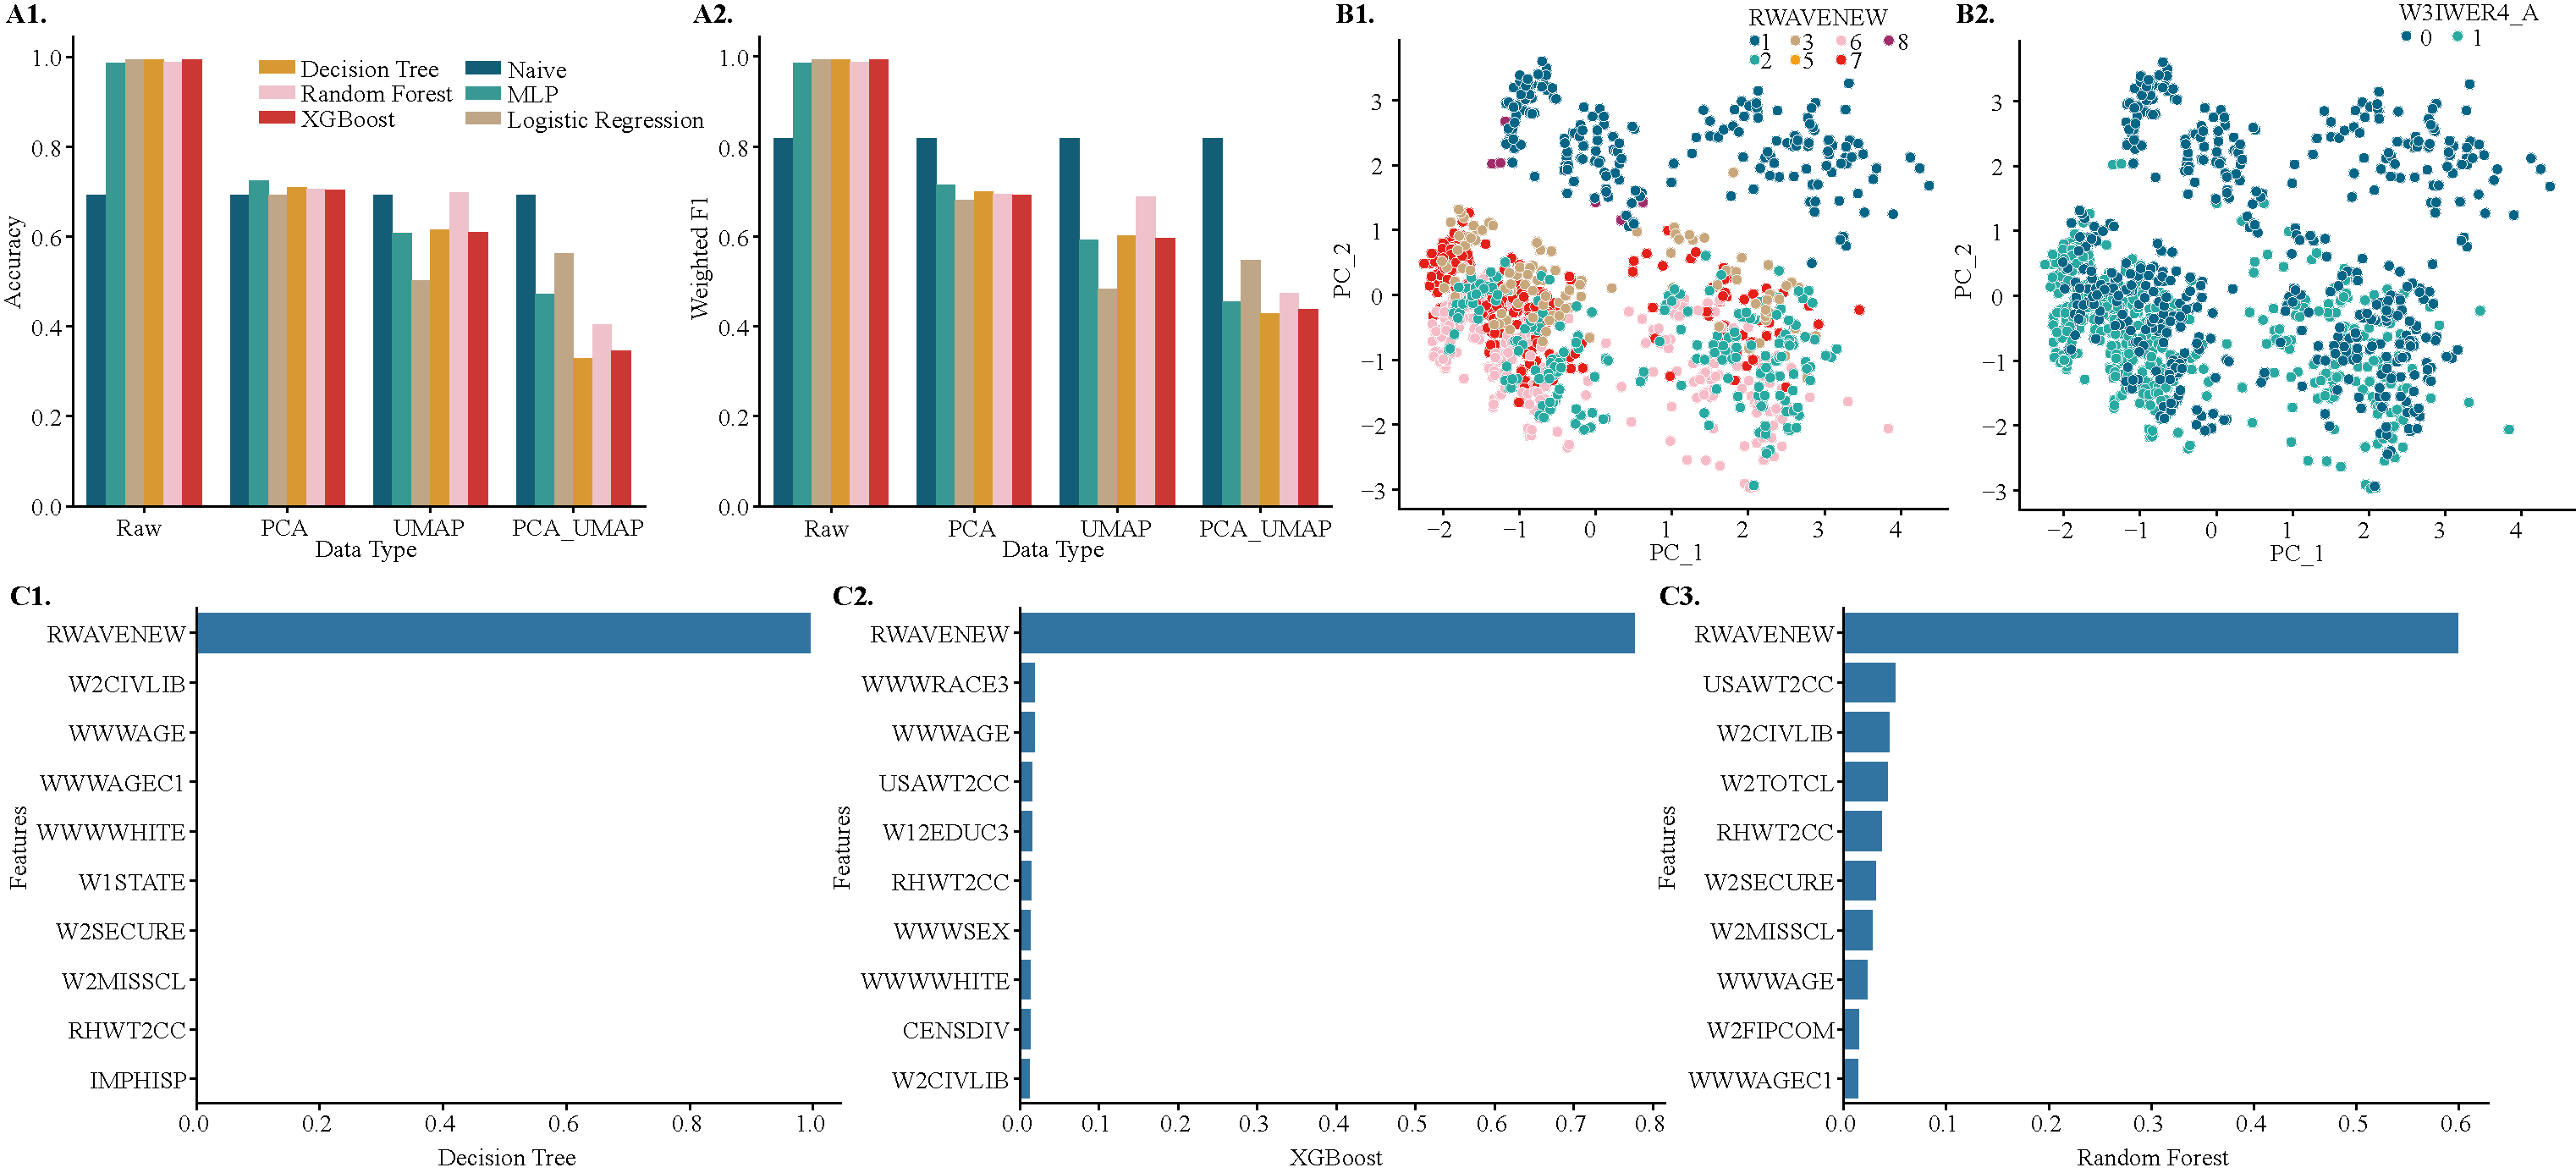
\includegraphics[width=\linewidth]{Figures/Figure2.pdf}
    \caption{Experimental results for batch effects exploration. Shown are the bar plots of test (A.1) accuracy and (A.2) weighted F1 score of the prediction of six classifiers with four data types, scatter plots of two dimensional principal components of the training dataset labelled by the (B1.) batch and (B2.) label, and horizontal bar plots of the training feature importance obtained by the (C1.) Decision Tree, (C2.) XGBoost, and (C3.) Random Forest. Top 10 features are retained. }
    \label{fig:figure2}
\end{figure*} 

\begin{figure*}[t!]
    \centering
    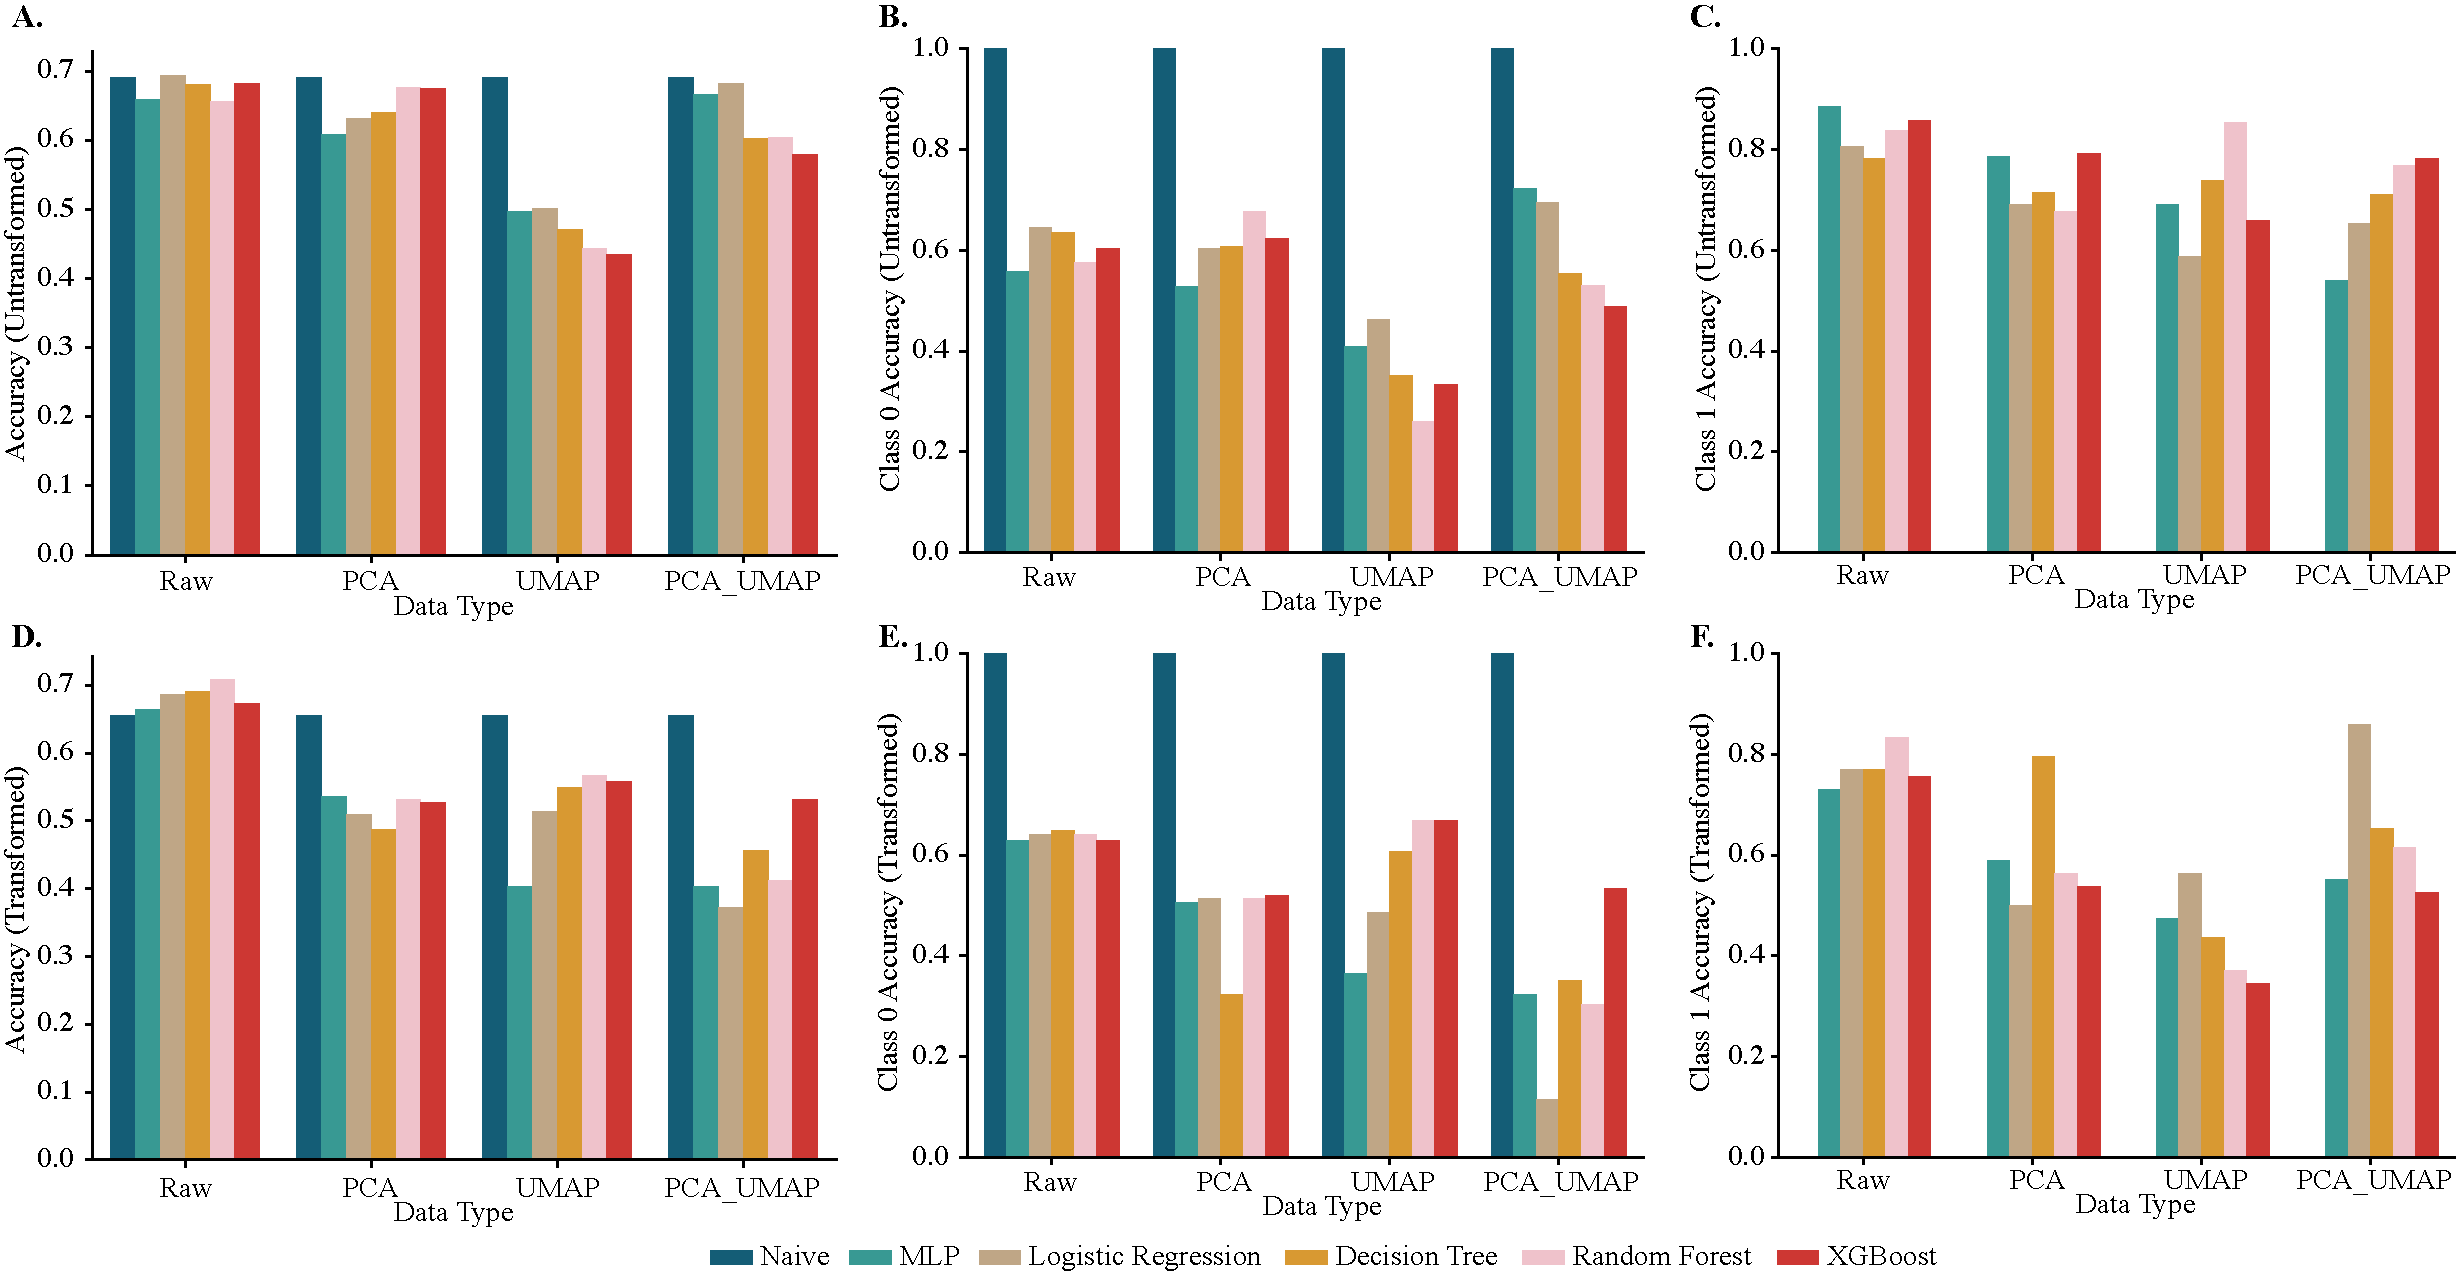
\includegraphics[width=14cm]{Figures/Figure3.pdf}
    \caption{Baseline experimental results. Shown are the bar plots of (A, D) test accuracy, (B, E) class 0 accuracy, (C, F) class 1 accuracy of the (top) untransformed and (bottom) transformed data. Each plot contains classification performance of six classifiers including naive approach with four data types.}
    \label{fig:figure3}
\end{figure*} 

\begin{figure*}[t!]
    \centering
    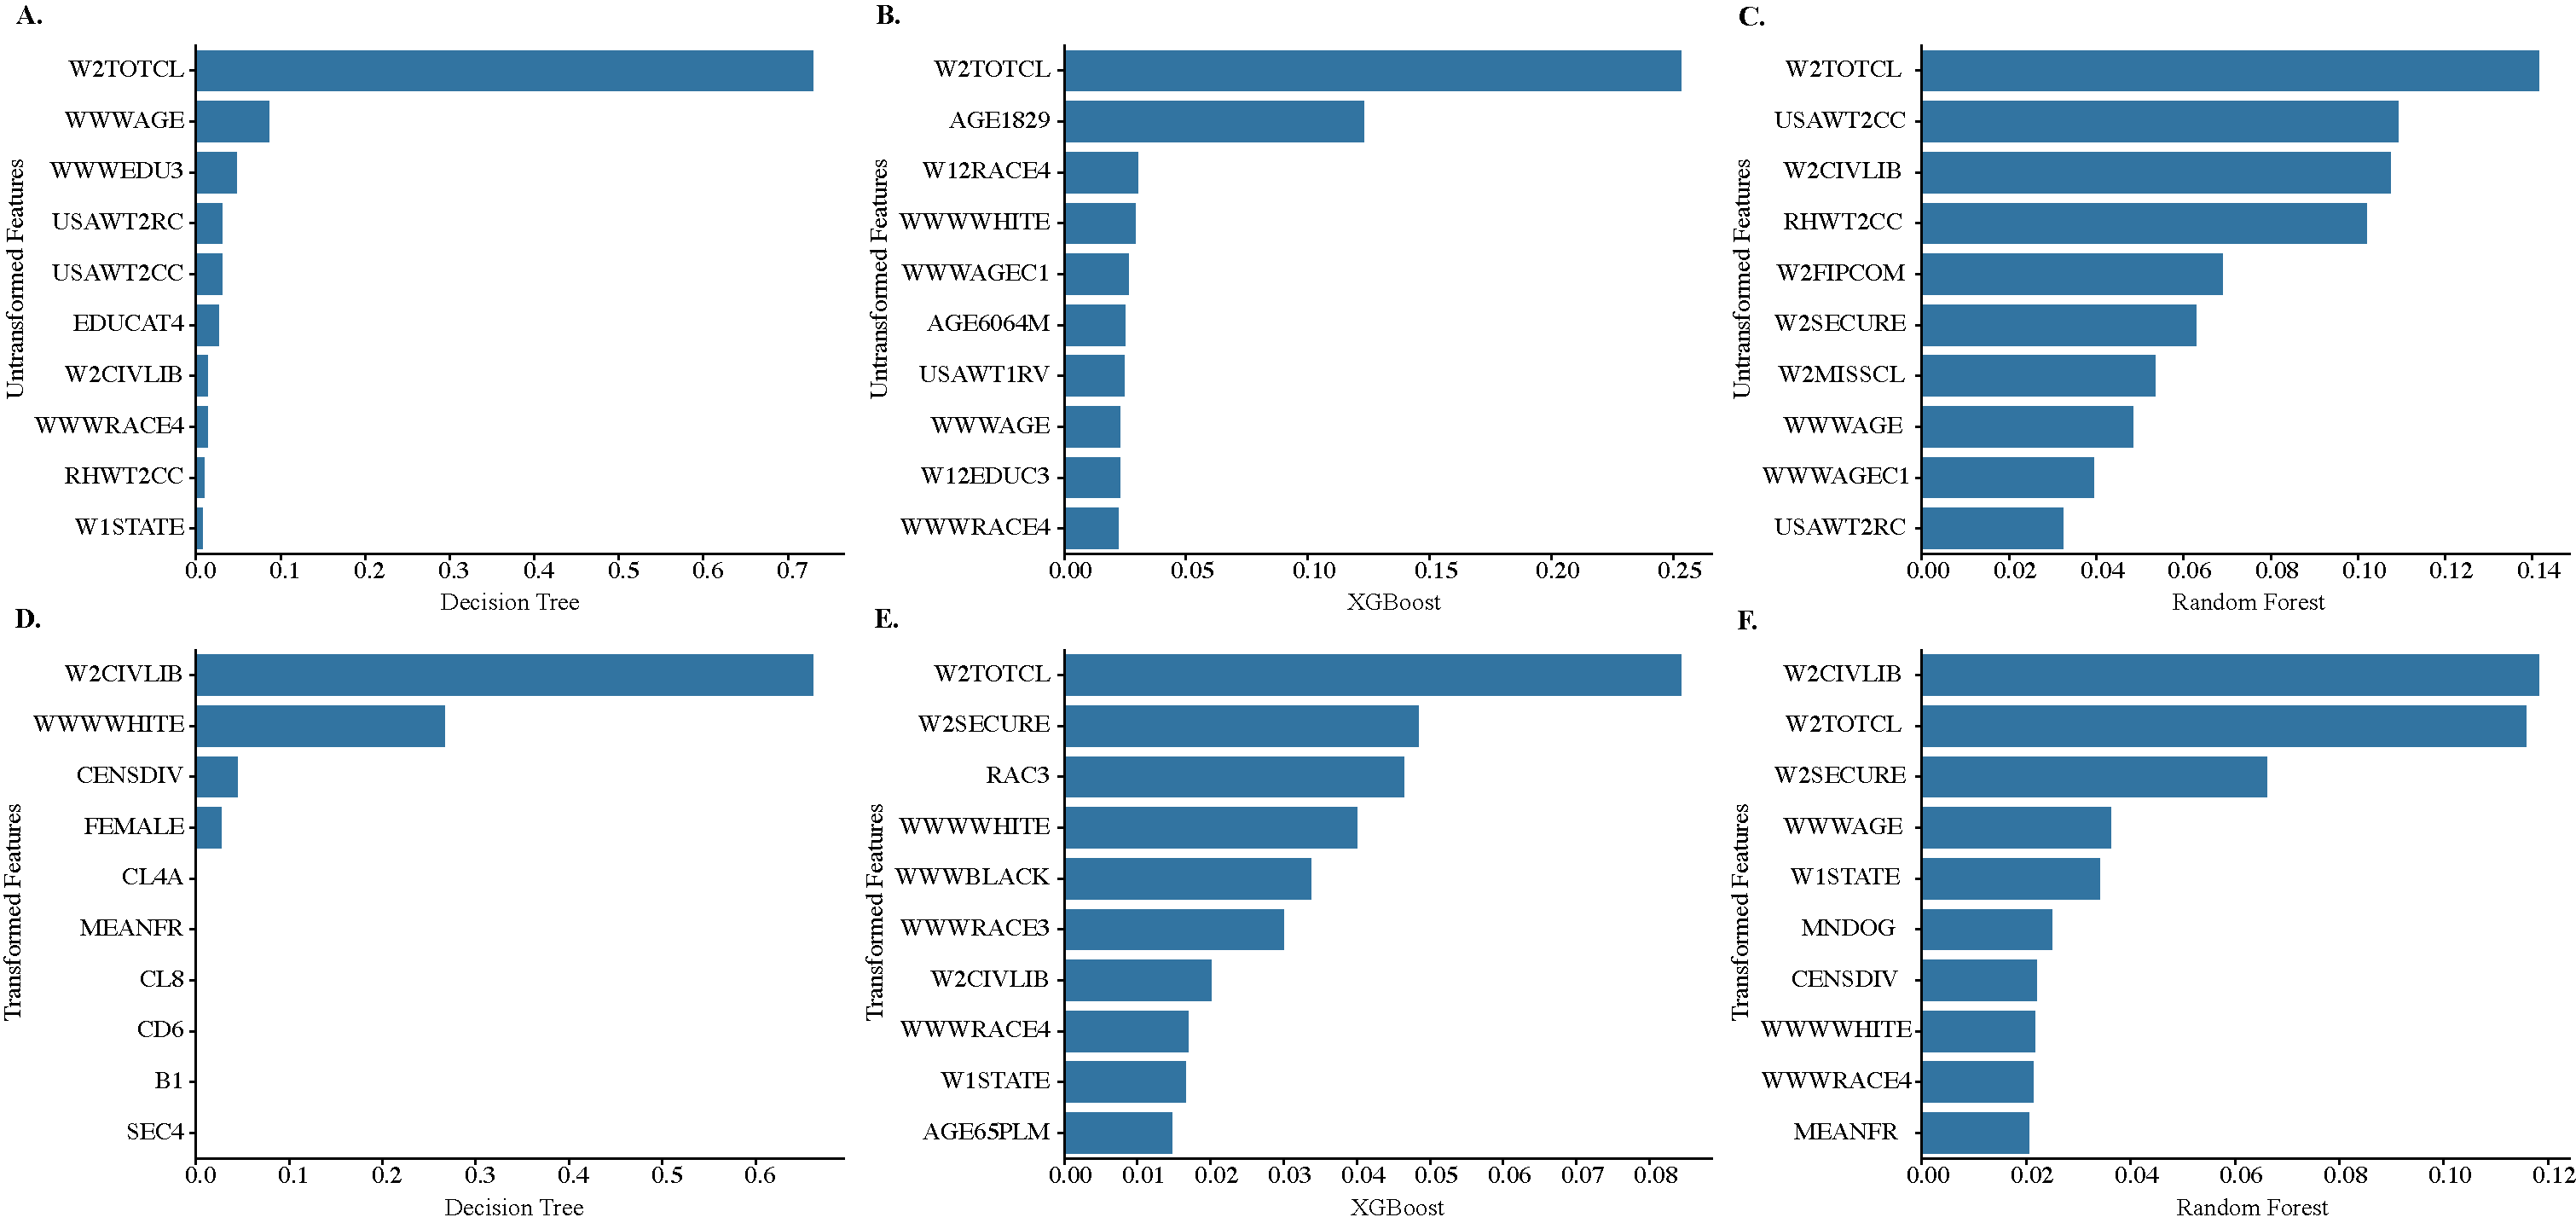
\includegraphics[width=14cm]{Figures/Figure4.pdf}
    \caption{Feature importance for baseline experiments. Shown are the horizontal bar plots of the feature importance of (top) untransformed and (bottom) transformed data predicted by (left) Decision tree, (middle) XGBoost, (right) Random Forest.}
    \label{fig:figure4}
\end{figure*} 

\begin{figure*}[t!]
    \centering
    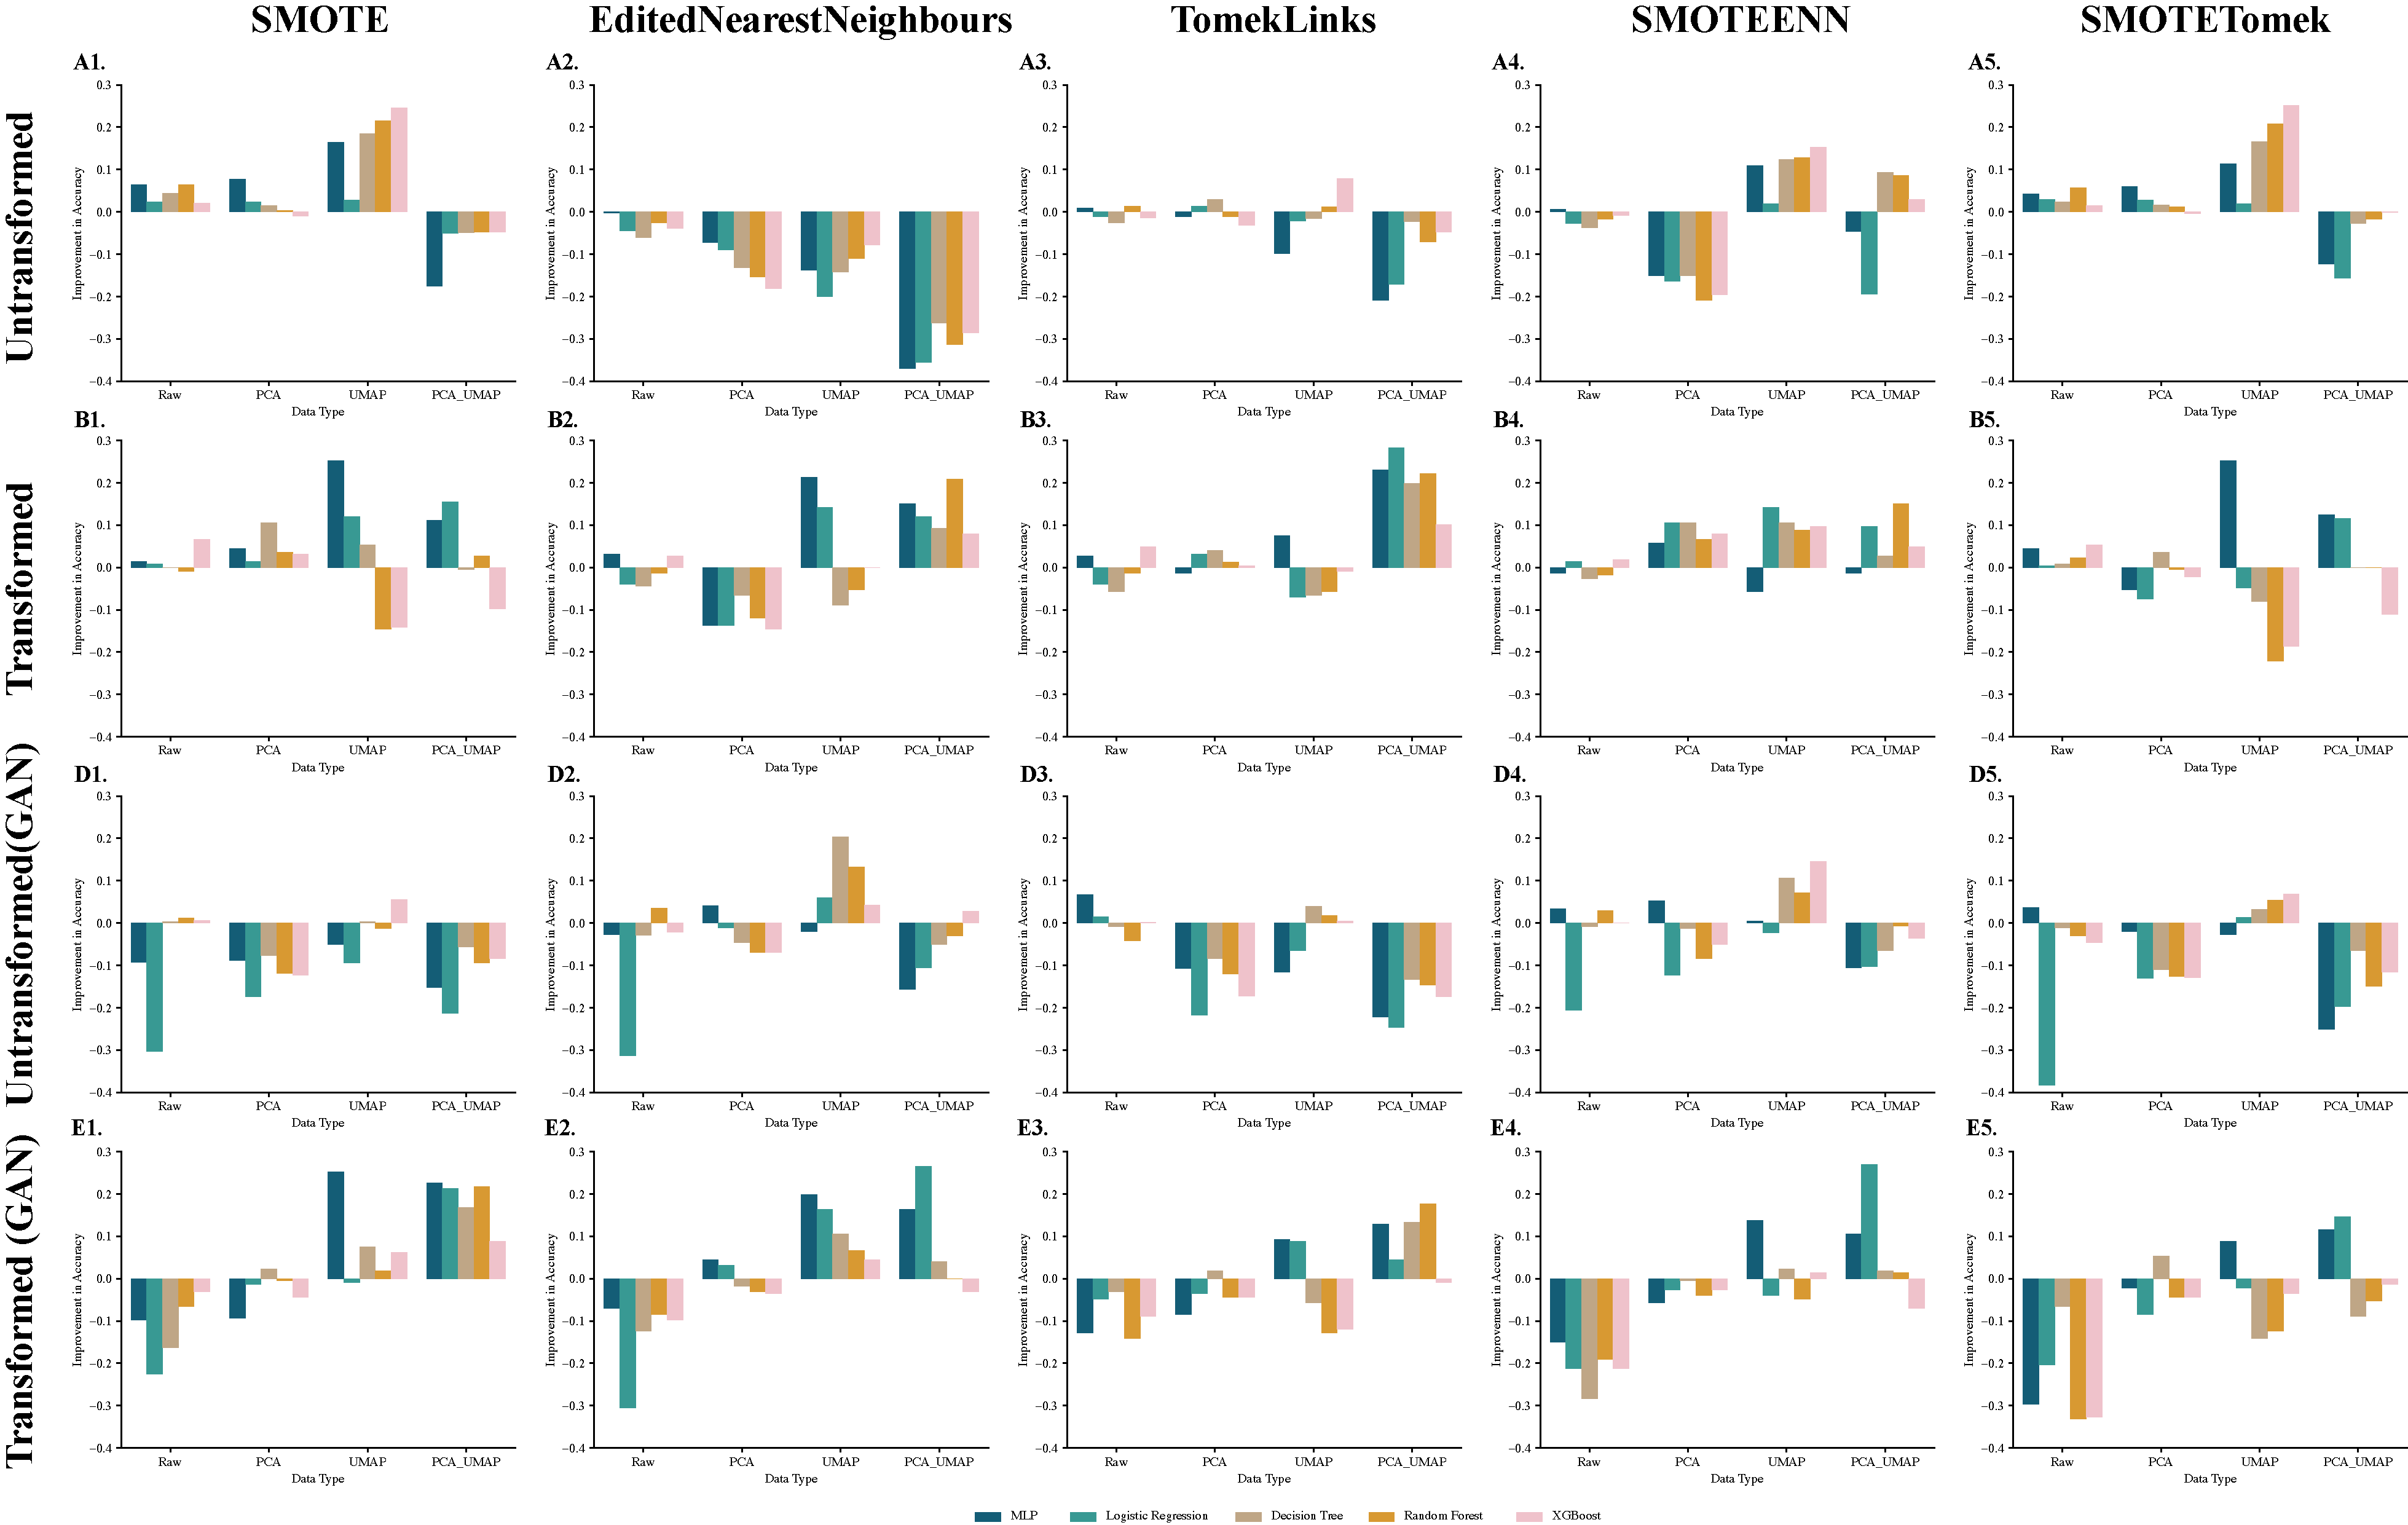
\includegraphics[width=\linewidth]{Figures/Figure5.pdf}
    \caption{Results for benchmarking data augmentation methods. Shown are the bar plots of the improvement in accuracy after applying data augmentation methods compared to the baseline results. Five sampling data augmentation methods are tested with (A.) untransformed data and (B.) transformed data. (C.) and (D.) demonstrated the improvement in performance after augmenting GAN to each of the sampling-based data augmentation method with untransformed and transformed data, respectively.}
    \label{fig:figure5}
\end{figure*}

The results demonstrate the flexibility and easy use of the framework to explore meaningful patterns, provide baseline results, and benchmark data augmentation methods. We found two variables which caused batch effects in our dataset. Using our proposed data transformation method, we show that our method is well suited to resolve batch effect without sacrificing performance. Our method also provides more meaningful interpretations, where we have empirically shown that data augmentation methods can improve the performance of classifiers for some datasets. For each of the experiment, we include datasets with four data types (Raw, PCA, UMAP, and PCA\_UMAP).

\textbf{A batch effect by wave-related variable is discovered.} When classifying the cooperativeness of the respondents from the original data features. We found that the performance of each classifiers is unreasonably high with raw data, where the average accuracy is 0.993$\pm$0.405 and the weighted F1 is 0.991$\pm$0.404 (figure ~\ref{fig:figure2}A). With such a phenomena, we suspected that batch effects might exist that affect the decision boundary of the classifiers. We therefore, computed the training feature importance of each feature by Decision Tree, XGBoost, and Random Forest (figure ~\ref{fig:figure2}C). We found a dominating variable RWAVENEW whose feature importance is significantly higher than the rest of the features. The variable RWAVENEW indicates the wave of the survey the respondents have participated in, and it seems that an inherent cluster exist by the RWAVENEW variable that guides the learning of classifiers. We confirmed our findings by creating the scatter plot of the training data labelling by the suspected variable and the training label (figure ~\ref{fig:figure2}B). The results demonstrate that an cluster exist in the training that is not only based on the label but also on the batch RWAVENEW. Interestingly, after dimensionality reduction, the effect of batch effects is slightly mitigated as a significant drop in performance could be observed in any of PCA, UMAP, or PCA\_UMAP data. We hypothesize that this behavior might be due to dimensionality reduction techniques that reduce the noises of the batch variable and make them less standing out in lower dimensions.

Since the purpose of this study is to find the cooperativeness of the respondents solely from their answers, we classify this phenomenon as a batch effect by the wave-related variable. We further examined our dataset and found a variable RWAVEOLD that is highly correlated to RWAVENEW, and it generated similar results to RWAVENEW. Therefore, to remove batch effects we remove RWAVENEW and RWAVEOLD in rest of our experiments, where the dataset is called untransformed dataset. In addition, since the dataset contains responses from three waves, we also proposed a data transformation method that further mitigates the batch effect by only obtaining the variables of the first wave that the respondents are interview in, which reduces the dimensionality, where the dataset is called transformed data. 

In rest of the experiments, we tested on different combination of both untransformed and transformed data with different data types. In addition, since weighted F1 generates similar patterns to accuracy and we still want to consider each class equally though a class imbalance exists in the testing data, we only use accuracy and class accuracy to evaluate the performance of classifiers.

\textbf{The proposed data transformation method could provide a more meaningful explanation to the features contributing to the prediction of cooperativeness while not sacrificing the performance.} The results demonstrating that the average classification accuracy across 5 classifiers not including naive classifier is not significantly different, where the averaged accuracy of prediction is 0.674 $\pm$ 0.163 on untransformed data and is 0.684 $\pm$ 0.0917 for transformed data (figure \ref{fig:figure3} AD). Although the class imbalance of testing data is different from transformed and untransformed data, the performance of 5 classifiers outperforms the naive classifier and demonstrates the superiority of transformed dataset in its own context. However, the performance of classifiers in transformed dataset drops significantly compared to the untransformed dataset except for UMAP, where the average accuracy (0.518 $\pm$ 0.067) of transformed data in UMAP significantly outperforms the average accuracy (0.469 $\pm$ 0.030) of untransformed data in UMAP, demonstrating that a non-linear reduction technique might be better at capturing the internal data structure in the transformed data. Whereas, in untransformed data, interestingly, PCA reduction and PCA\_UMAP reduction does not significantly decrease the performance of classifiers except for UMAP reduction, indicating that a linear relationship exist in the dataset that if one wants to use a dimensionality reduction technique to reduce the features, a linear relationship must be captured.

In addition,, the classification accuracy of class 1 (figure \ref{fig:figure3} BE) which is the label cooperative is significantly higher than the classification accuracy of class 0 (figure \ref{fig:figure3} CF) which is the label uncooperative. The label cooperative is the minority class in the testing dataset and we hypothesize that in the testing data, a cluster might exist based on the label of cooperative which makes classifier easier to distinguish compared to uncooperative. A more detailed technical attribution is presented in discussion section. Additionally, the results show that tree-based classifiers are better at classifying the uncooperative except for a significantly high performance by logistic regression in transformed data with PCA\_UMAP reduction.

The transformed dataset produces more meaningful explanations of the feature importances since the models were not dominated by one feature. In the models trained on untransformed data in figure ~\ref{fig:figure4} ABC, W2TOTCL is far and above the most important feature in each model. In decision trees and XGBoost, W2TOTCL severely impacts the classification of a sample. In the models trained on transformed data in figure ~\ref{fig:figure4} DEF, the drop off in feature importance after the most influential features is much less. Although the decision tree is still dominated by one attribute, in XGBoost a significant scale shift is observed. For the XGBoost model trained on transformed data the most important feature importance was about 0.08; whereas, for the XGBoost model trained on the untransformed data the most important feature was about 0.25.

It is worth noting that the feature which models A, B, and C identify as the most influential feature for whether a respondent takes the survey seriously appears to be an example of overfitting. Models A, B, and C all identify W2TOTCL as the most important feature; however, this feature tracks how many questions a respondent favored civil-liberties in. Since the models appear to be overfitting on W2TOTCL, they are under-valuing the importance of other features yielding a less meaningful interpretation of feature importances. In the Discussion section, we will further explain why we believe our models trained on untransformed data to be overfitting.

\textbf{Data augmentation methods improve performance with low-dimensional training data, and the best classifier for classifying the cooperativeness of survey respondent is created by augmented and transformed training data.} In general, data augmentation methods are more effective in UMAP (0.03$\pm$0.118) and PCA\_UMAP (-0.0119$\pm$ 0.148) data compared to Raw (-0.05$\pm$0.103) and PCA (-0.04$\pm$0.075) data by improvement in accuracy across all data and methods (figure ~\ref{fig:figure5}). Despite the negative overall improvement in PCA\_UMAP data, its large standard deviation suggests that the augmentation methods are indeed effective in most of the dataset for PCA\_UMAP data. Considering UMAP and PCA\_UMAP data, SMOTE (0.035$\pm$0.130) and SMOTENN (0.040$\pm$0.090) are the best data augmentation methods having top two improvements in accuracy. However, GAN is not effective when augmenting to each of the sampling-based data augmentation methods except for editENN with a average improvement in accuracy of 0.056$\pm$0.107 across both transformed and untransformed data. We attributed this behavior to the over down-sampling by the editENN as it can be observed from figure ~\ref{fig:figure5} A2. where editENN significantly drops the performance. Therefore, by increasing the size of the training data, GAN is more effective when augmented with the editENN. Although across transformed and untransformed data, GAN is not effective in improving the performance, it performs differently in transformed data than untransformed data. In transformed data, GAN improves the average accuracy by 0.060$\pm$0.108 compared to the -0.045$\pm$0.102 of untransformed data. The reason is that after transformation, the size of the training data is significantly smaller than the size of training data with untransformed data as shown in table ~\ref{tab:table1}.

After data augmentation, combining baseline performance, the best classifier is XGB with raw, transformed, and augmented data, having a accuracy of 0.739 (table ~\ref{tab:table2}). Interestingly, the top two classifiers both take transformed data as input, and both of the classifiers use augmented training data. Therefore, we conclude that the performance of classifiers in classifying cooperativeness in survey is improved by applying data transformation and augmentation techniques. 





\section{Discussion}
\begin{figure}[ht!]
    \centering
    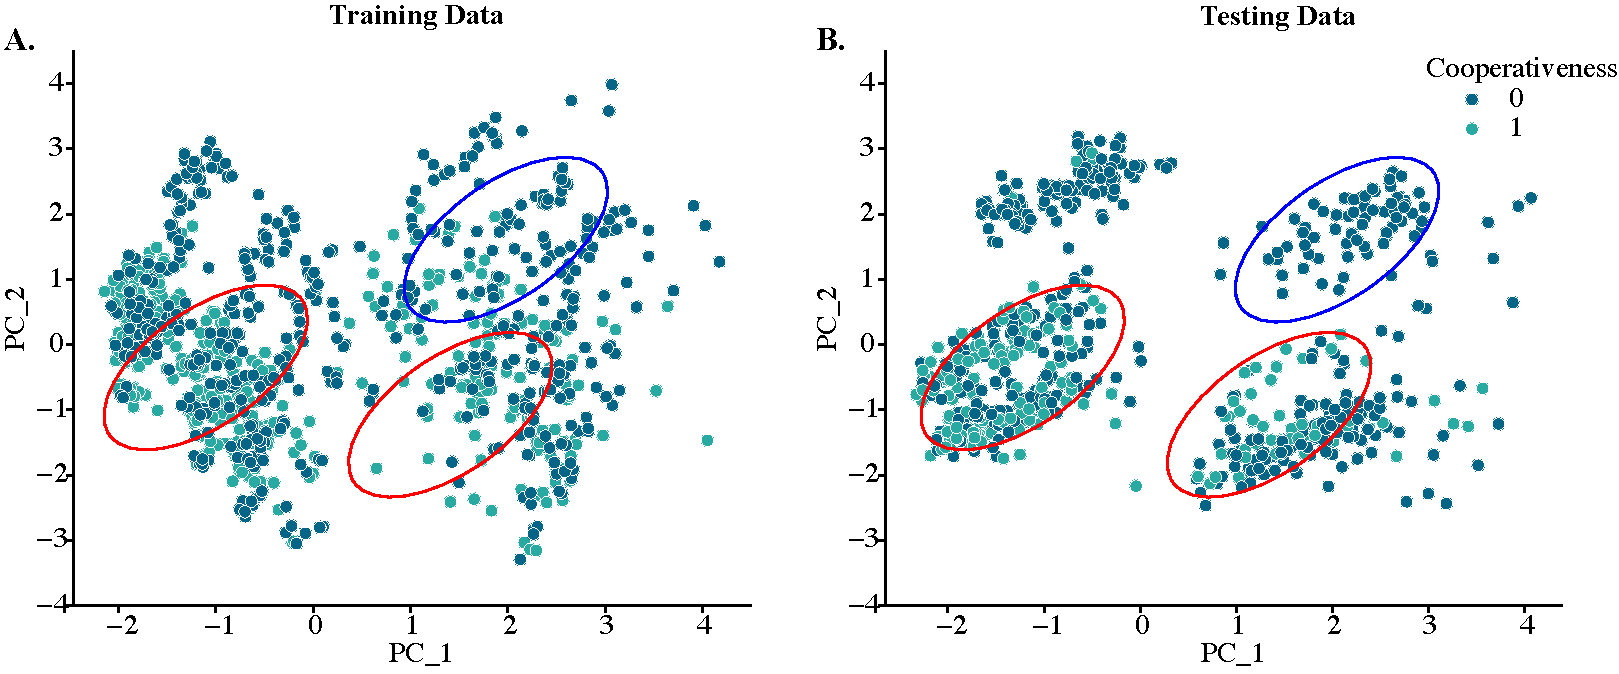
\includegraphics[width=\linewidth]{Figures/Figure6.pdf}
    \caption{Exploration of Accuracy Imbalance. Shown are the scatter plots of untransformed two principal components of (A.) training data and (B.) testing data.}
    \label{fig:figure6}
\end{figure} 

During our preliminary exploration of the data, we clustered the dataset, balancing respect to a respondents preference for civil-liberty or security-based policy. Although there appeared to be underlying trends in the data, the cluster algorithms employed were unable to separate the data on civil-liberty or security-based policy. Our suspicion was that there were untrustworthy samples in the dataset since some clusters were almost pure outside of a few mislabeled samples. Upon further inspection of the dataset, we confirmed our suspicions that some data points were higher fidelity than others. A large number of samples contained low cooperation scores by the interviewer and others completed the survey in unreasonable short time periods. This led us to our current research task of filtering out uncooperative samples in survey datasets to produce high fidelity datasets without sacrificing classification accuracy. 

Next we started developing a classifier to identify samples that contained high levels of cooperation as measured by the interviewer. At this stage we found that our dataset contains a particular form of data bias called batch effect. Batch effect occurs when data variations cause biases that make it challenging to identify the true causes of the relationship at play. In our case the two variables causing the batch effect were RWAVENEW and RWAVEOLD. RWAVENEW denotes if this is the first time a respondent is being surveyed and RWAVEOLD denotes if the respondent is a repeat survey participant. When training classifiers to predict cooperativeness of respondents RWAVENEW and RWAVEOLD drown out the feature importance of all the other features as can be seen in Figure 2. To address the batch effect, we removed both RWAVENEW and RWAVEOLD from our dataset. The result of removing RWAVEOLD and RWAVENEW can be seen in plots A, B, and C of Figure 3. In Figure 3, plots A, B, and C demonstrate more well rounded feature importances than those found in Figure 2. 

After removing the features causing the batch effect, we gathered out baseline feature importance from our classifiers. While these feature importances were more interpretable than our previous feature importances, all three classifiers overfit with respect to attribute W2TOTCL. In each classifier, as depicted in plots A, B, and C of Figure 3, W2TOTCL is by far the most important feature. However, when looking at the data and the context of our investigation this implies that a respondent's cooperation can be predicted based on whether they support civil-liberty based policy or not. Upon another round of inspecting the data, there is a reasonable explanation as to why these classifiers are finding this pattern. In the original dataset, out of those samples who were labeled cooperative, only 18\% answered a question where they favored civil liberties. However, for those respondents who did not take the survey seriously, 45\% of them answered a question where they favored civil liberties. 
	
To address the overfitting we initially faced, we designed a data transformation as described in Data Transformation and applied it to our dataset. Again, like when we removed the batch effect variables, the feature importances became less centralized in the most important features. Notably, two of our three classifiers trained on transformed data did not identify W2TOTCL as the most important feature. However, features strongly related to a particular preference for or against civil liberties policy were consistently influential. Our takeaway is that we continually improved the performance of the model but there is likely still overfitting in our classifiers. 

We explore more on the imbalanced accuracy in the baseline results. Interestingly, 0 which is uncooperative, is the majority class in the testing data, and the the testing accuracy supposes to be higher in uncooperative class. However, the testing accuracy of minority class is significantly higher than the other. We therefore suspect that something unexpected is happening in the feature space for the training and testing data. Through further investigation, first, we found that the testing data created by the stratified train-test split by sklearn can not fully capture the inherent data structure of the training data. From figure ~\ref{fig:figure6}, it is apparent that the train data has two clusters but the testing data has four clusters, where some information between the connection in top and bottom cluster is lost. Second, we discovered that the reason cooperative data is more identifiable in testing data is that they seem to form a cluster themselves in the testing data as indicated by the red circle, where in the training data, these circle contains majority of cooperative class. In addition, as indicated by the blue circle, some of the uncooperative class might be misclassified because in the training data, there are mixed uncooperative and cooperative class, which accounts for the low performance in the uncooperative class.

In benchmarking of data augmentation methods, we found that, data augmentation methods are more effective in training data with low dimensional features, and GAN is more effective with transformed data. We believed that since in low-dimensional data, each feature tends to carry more significance, and there's less noise compared to high-dimensional data, data augmentation in such a setting can effectively introduce meaningful variability without overwhelming the model with noise or irrelevant information. This helps the model learn the essential patterns more effectively. In addition, in high-dimensional spaces, up-sampling or down-sampling becomes much more challenging due to the curse of dimensionality because most of the sampling based data augmentation methods involve calculating distance. Additionally, the purpose of augmenting a GAN after sampling-based augmentation methods is to increase the training size. Therefore, it is reasonable that GAN is more effective in transformed data since from table ~\ref{tab:table1}, data after transformed has significantly less samples after processing compared to the untransformed data. That also accounts for why GAN improves the performance after applying editENN since editENN generates a small training dataset compared to other methods. 
\section{Conclusion}
In this study we investigated how to classify uncooperative survey respondents based on using classifiers, while employing data augmentation and CRISP-DM design principles. The main contributions of our study include: an automated user-friendly framework for benchmarking data augmentation methods and generating high fidelity training data, a classifier that predicts respondents cooperativeness to being surveyed with high performance, and a transformation method that mitigates the batch effects. We conclude that data augmentation methods are in fact useful for identifying untrustworthy survey data since they can differentiate classification differences and can provide better representation of under-surveyed populations. Our work contributes to the broader goal of developing high fidelity tabular dataset from survey response, a task that many information companies and researchers face today. In future work, cross analyzing our methods with another dataset would strengthen our conclusion that data augmentation should be used to improve classification of untrustworthy survey data. 

%\balance %balance the last two columns
\bibliographystyle{ACM-Reference-Format}
\bibliography{CSC673_Assignment6/reference} 
\end{document}
\endinput
